\part{Convolutions-and-Laplace-Transforms}
\lecture{Convolutions and the Laplace Transform}{Convolutions-and-the-Laplace-Transform}
\section{Convolutions and the Laplace Transform}

\title{Ordinary Differential Equations}
\subtitle{Convolutions and the Laplace Transforms}
\date{30 Nov 2012}

\begin{frame}
  \titlepage
\end{frame}

\begin{frame}
  \frametitle{Outline}
  \tableofcontents[pausesection,hideothersubsections]
\end{frame}


\subsection{The Convolution}


\begin{frame}
  \frametitle{Time Averaging}

  What if we want a ``time average'' based on the past? 

  \centerline{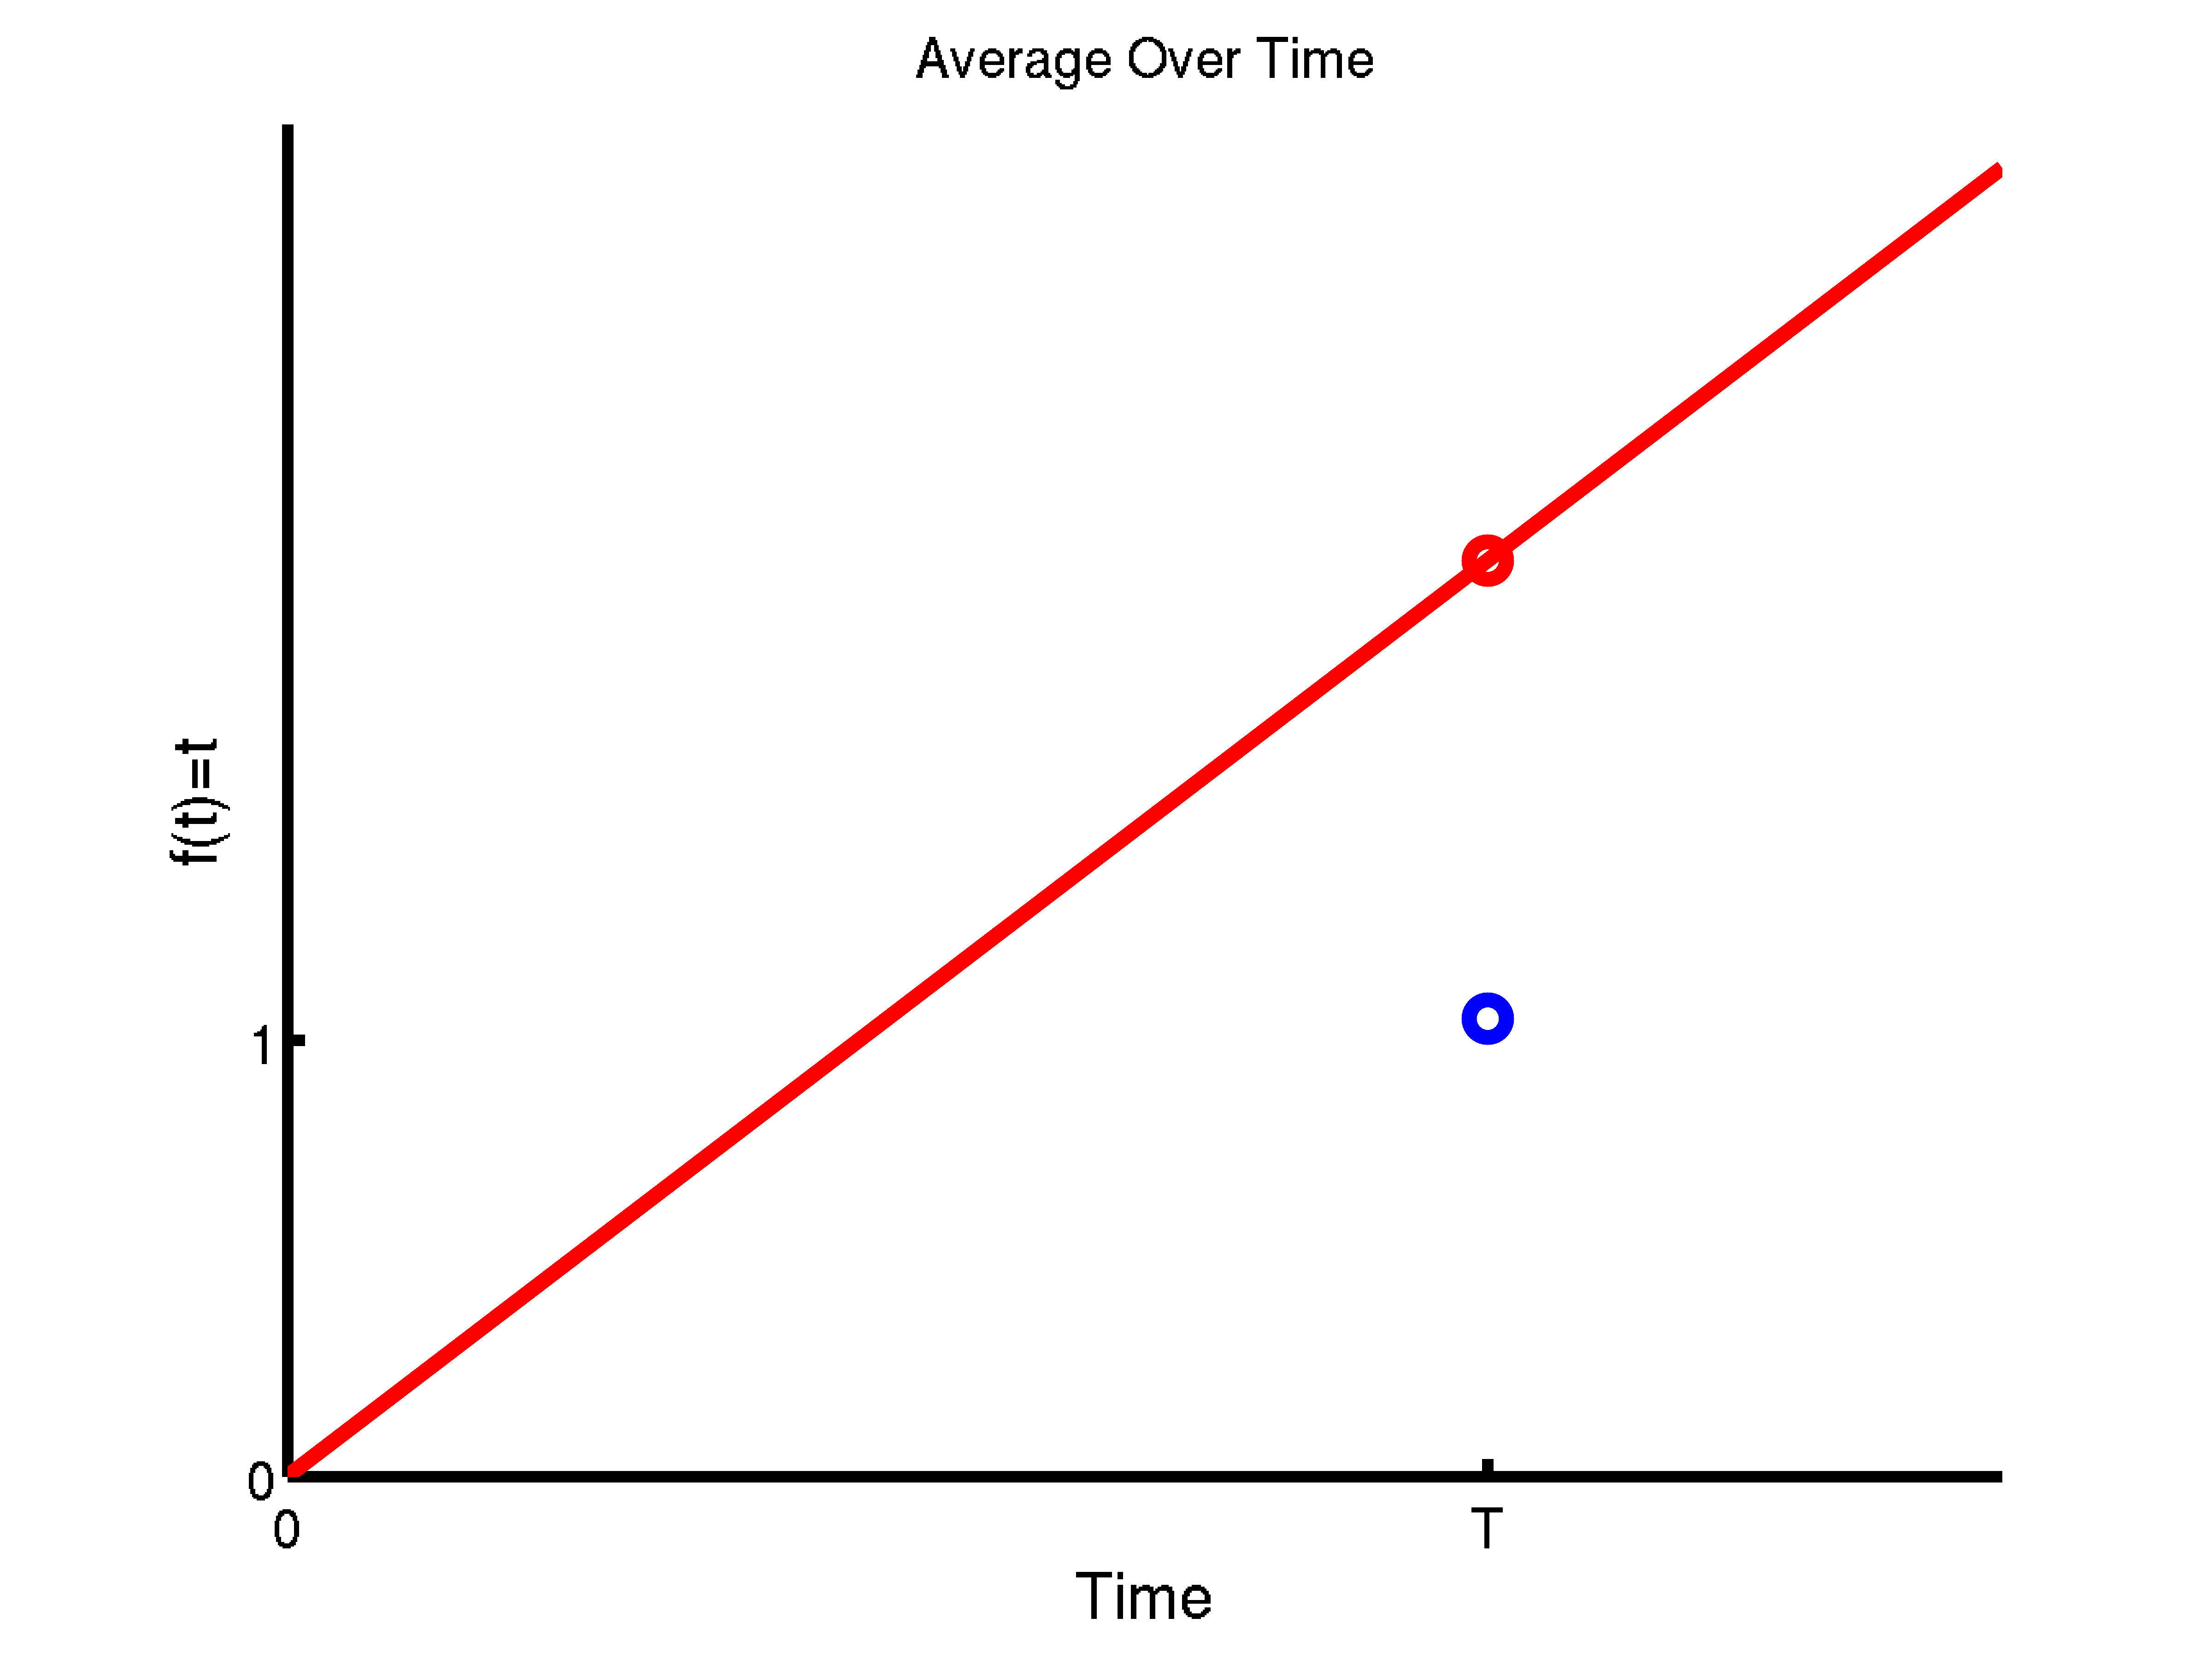
\includegraphics[width=4cm]{img/linearAverage}}

  \uncover<2->
  {%

    The effect of $f$ depends on what happened in the past. 
    In Calc II the average of a function from $0$ to $T$ was defined to be 
    \begin{eqnarray*}
      \frac{1}{T} \int^T_0 f(u) ~ du
    \end{eqnarray*}

  }


\end{frame}

\begin{frame}
  \frametitle{Time Averaging}

  \vspace*{-1em}
  What if we want a ``time average'' based on the past? \\
  \centerline{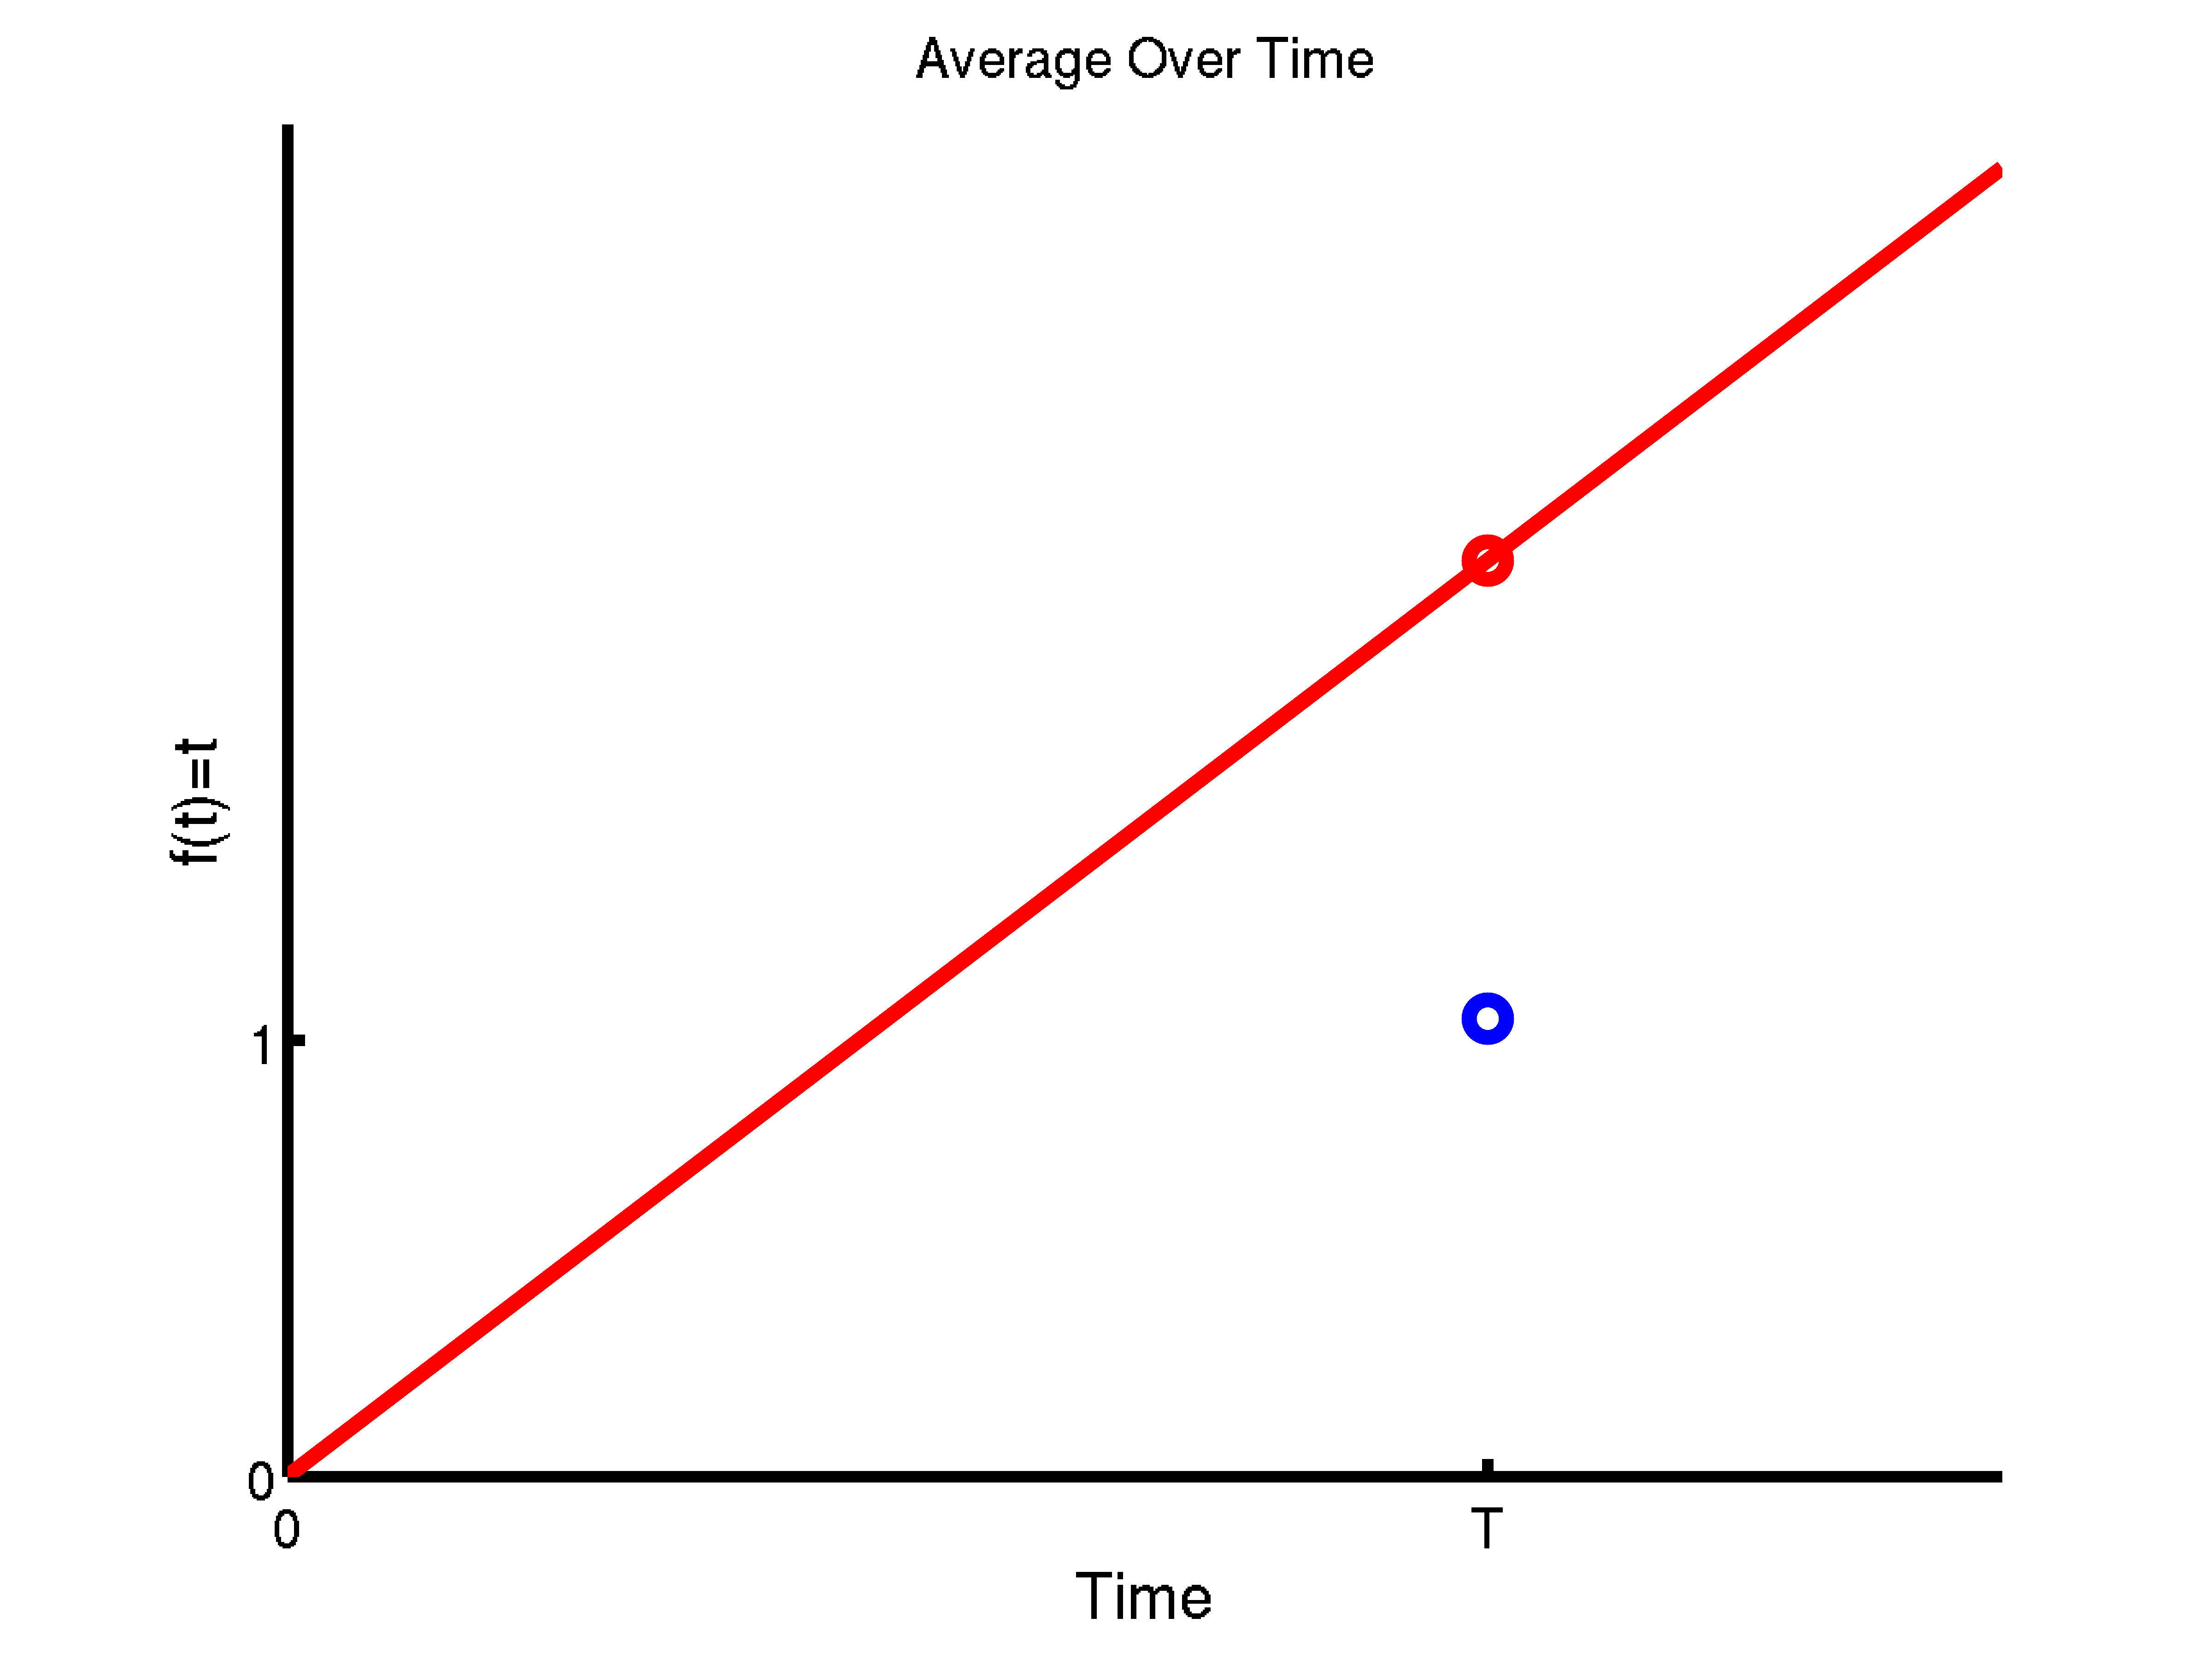
\includegraphics[width=4cm]{img/linearAverage}}

  Example: \\
  If $f(t)=t$, the average value is 
  \begin{eqnarray*}
    \frac{1}{T} \int^T_0 u ~ du & = & \half T
  \end{eqnarray*}

\end{frame}


\begin{frame}
  \frametitle{Time Averaging}

  \centerline{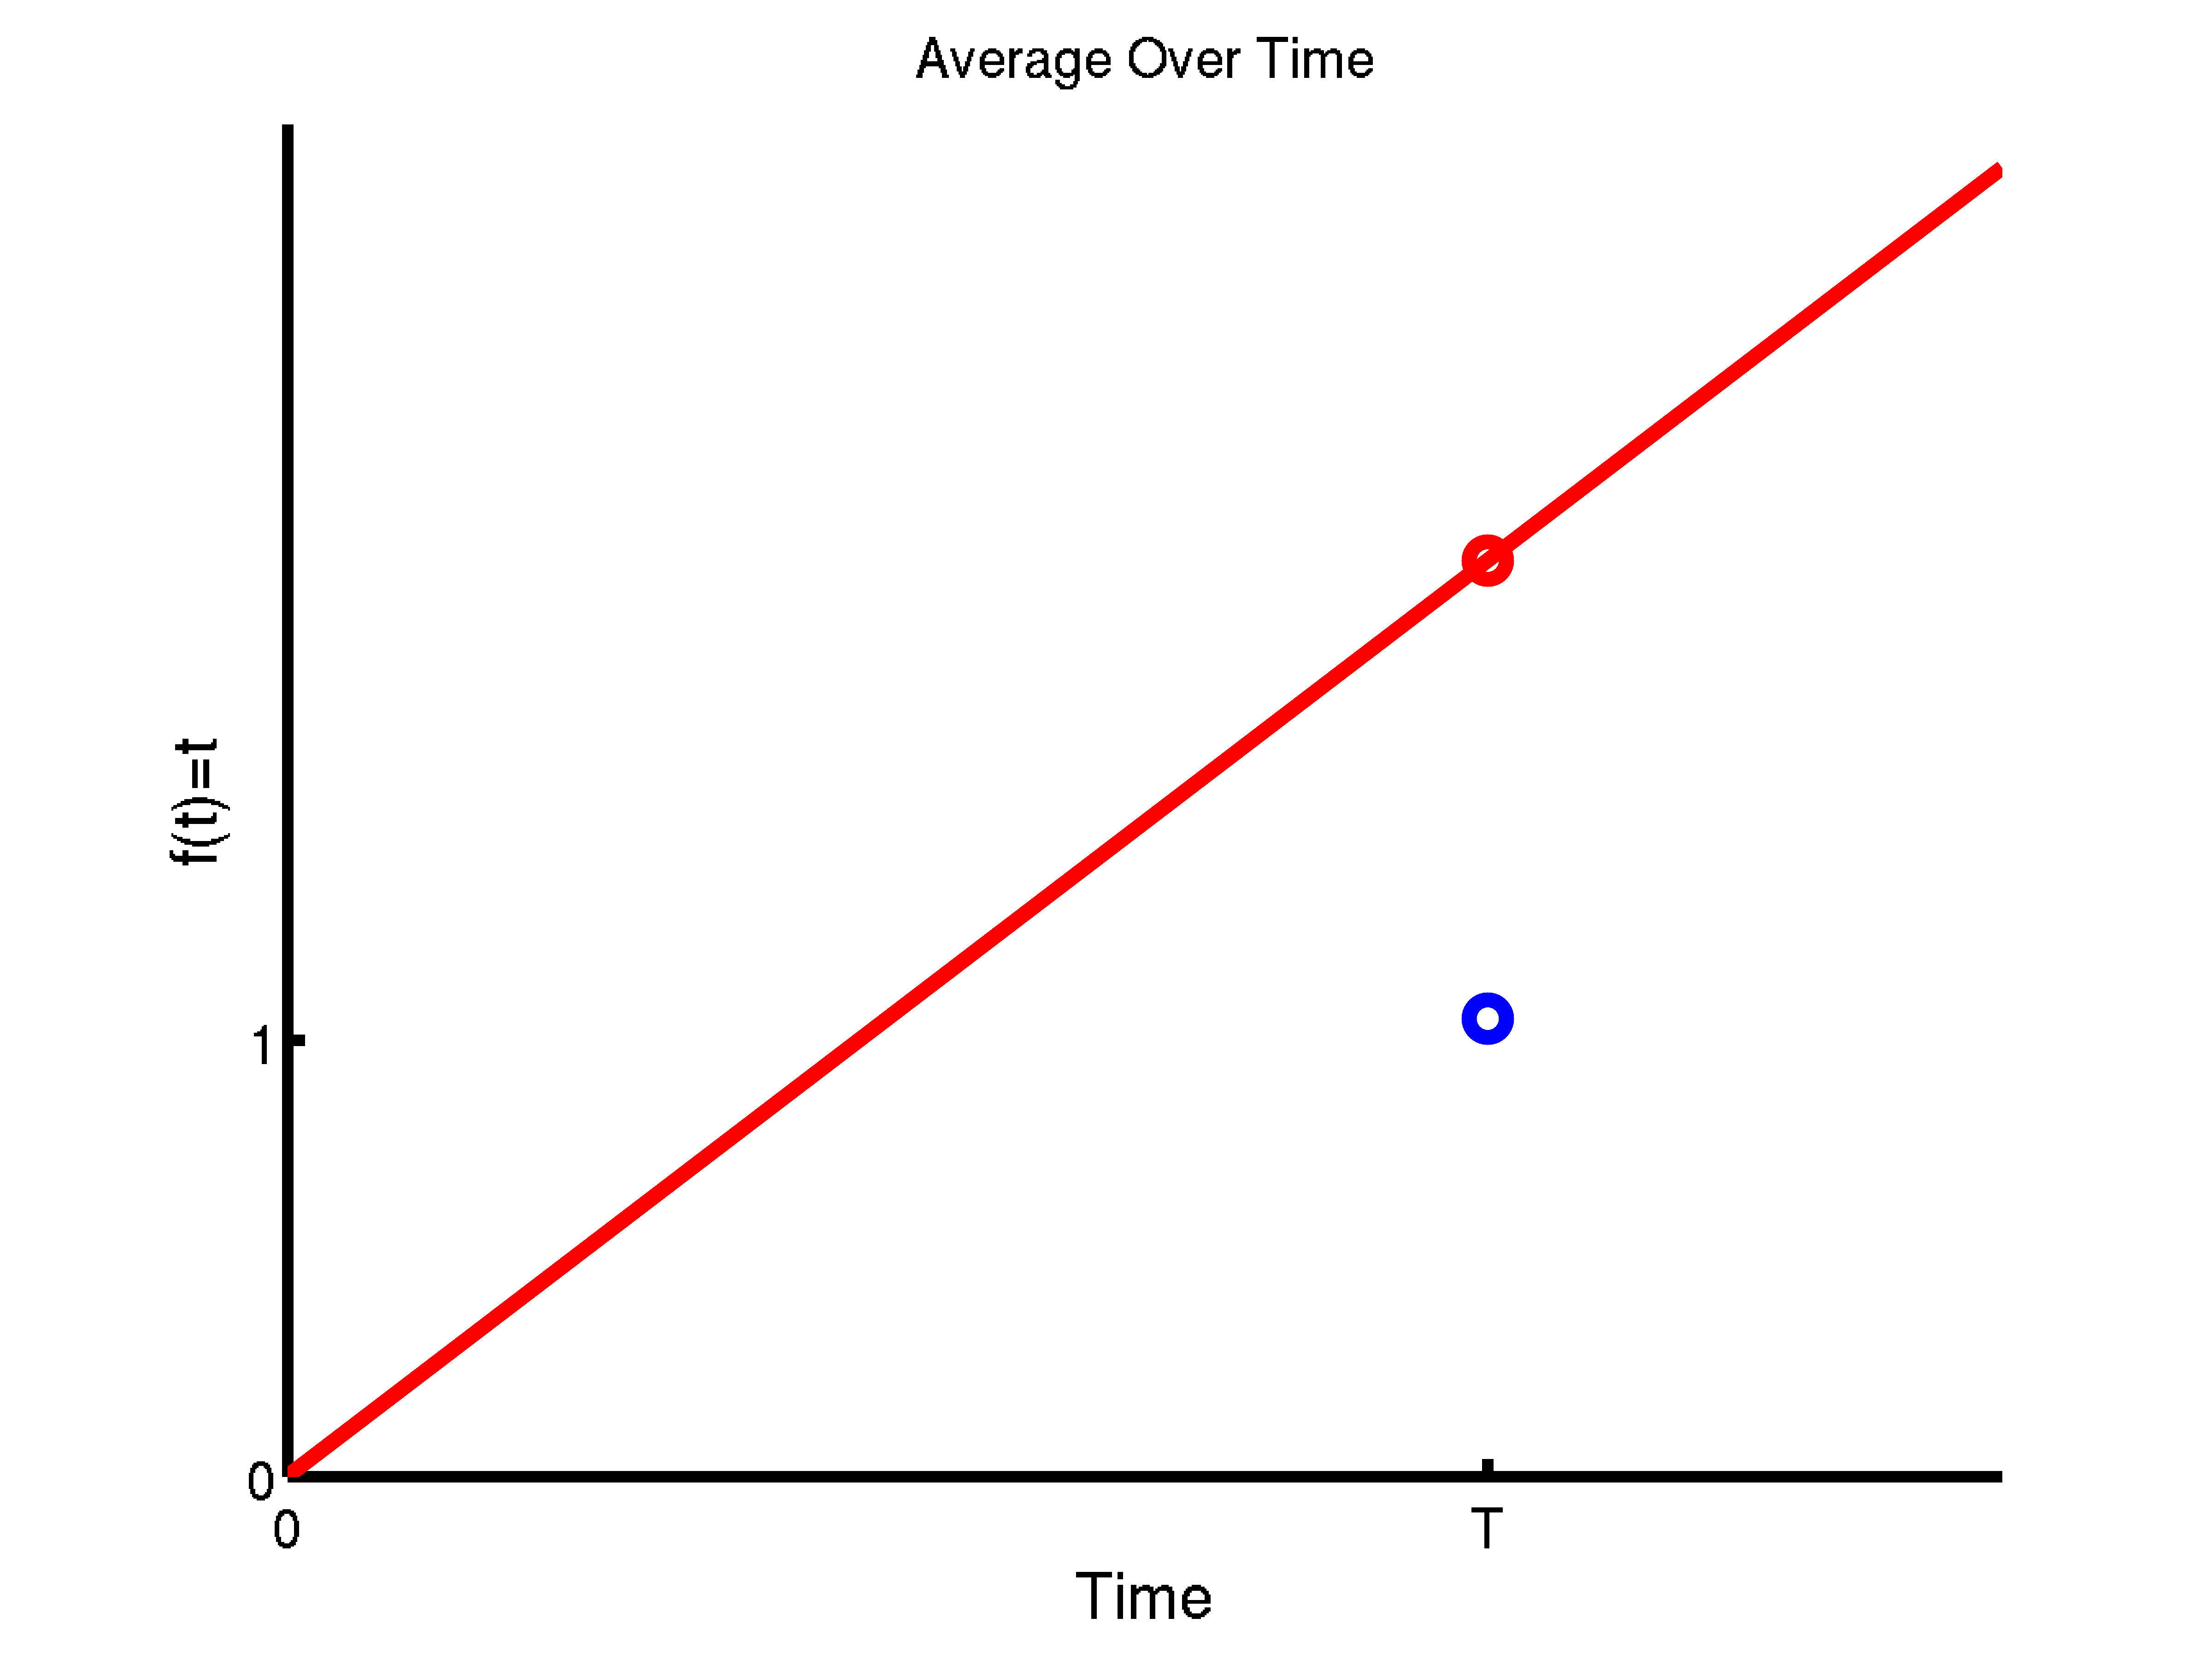
\includegraphics[width=5cm]{img/linearAverage}}

  Problem: \\
  All points in the past are equally ``weighted.'' What if the
  \textit{recent} is more important?

\end{frame}


\begin{frame}
  \begin{definition}
    Given two functions, $f$ and $g$, their convolution is defined to be
    \begin{eqnarray*}
      f*g & = & \int^t_0 f(t-w) g(w) ~ dw.
    \end{eqnarray*}
  \end{definition}
\end{frame}

\begin{frame}
  \frametitle{Translation}

  \begin{columns}

    \column{.5\textwidth}
    \vfill

    Note that given $f(t)$

    \centerline{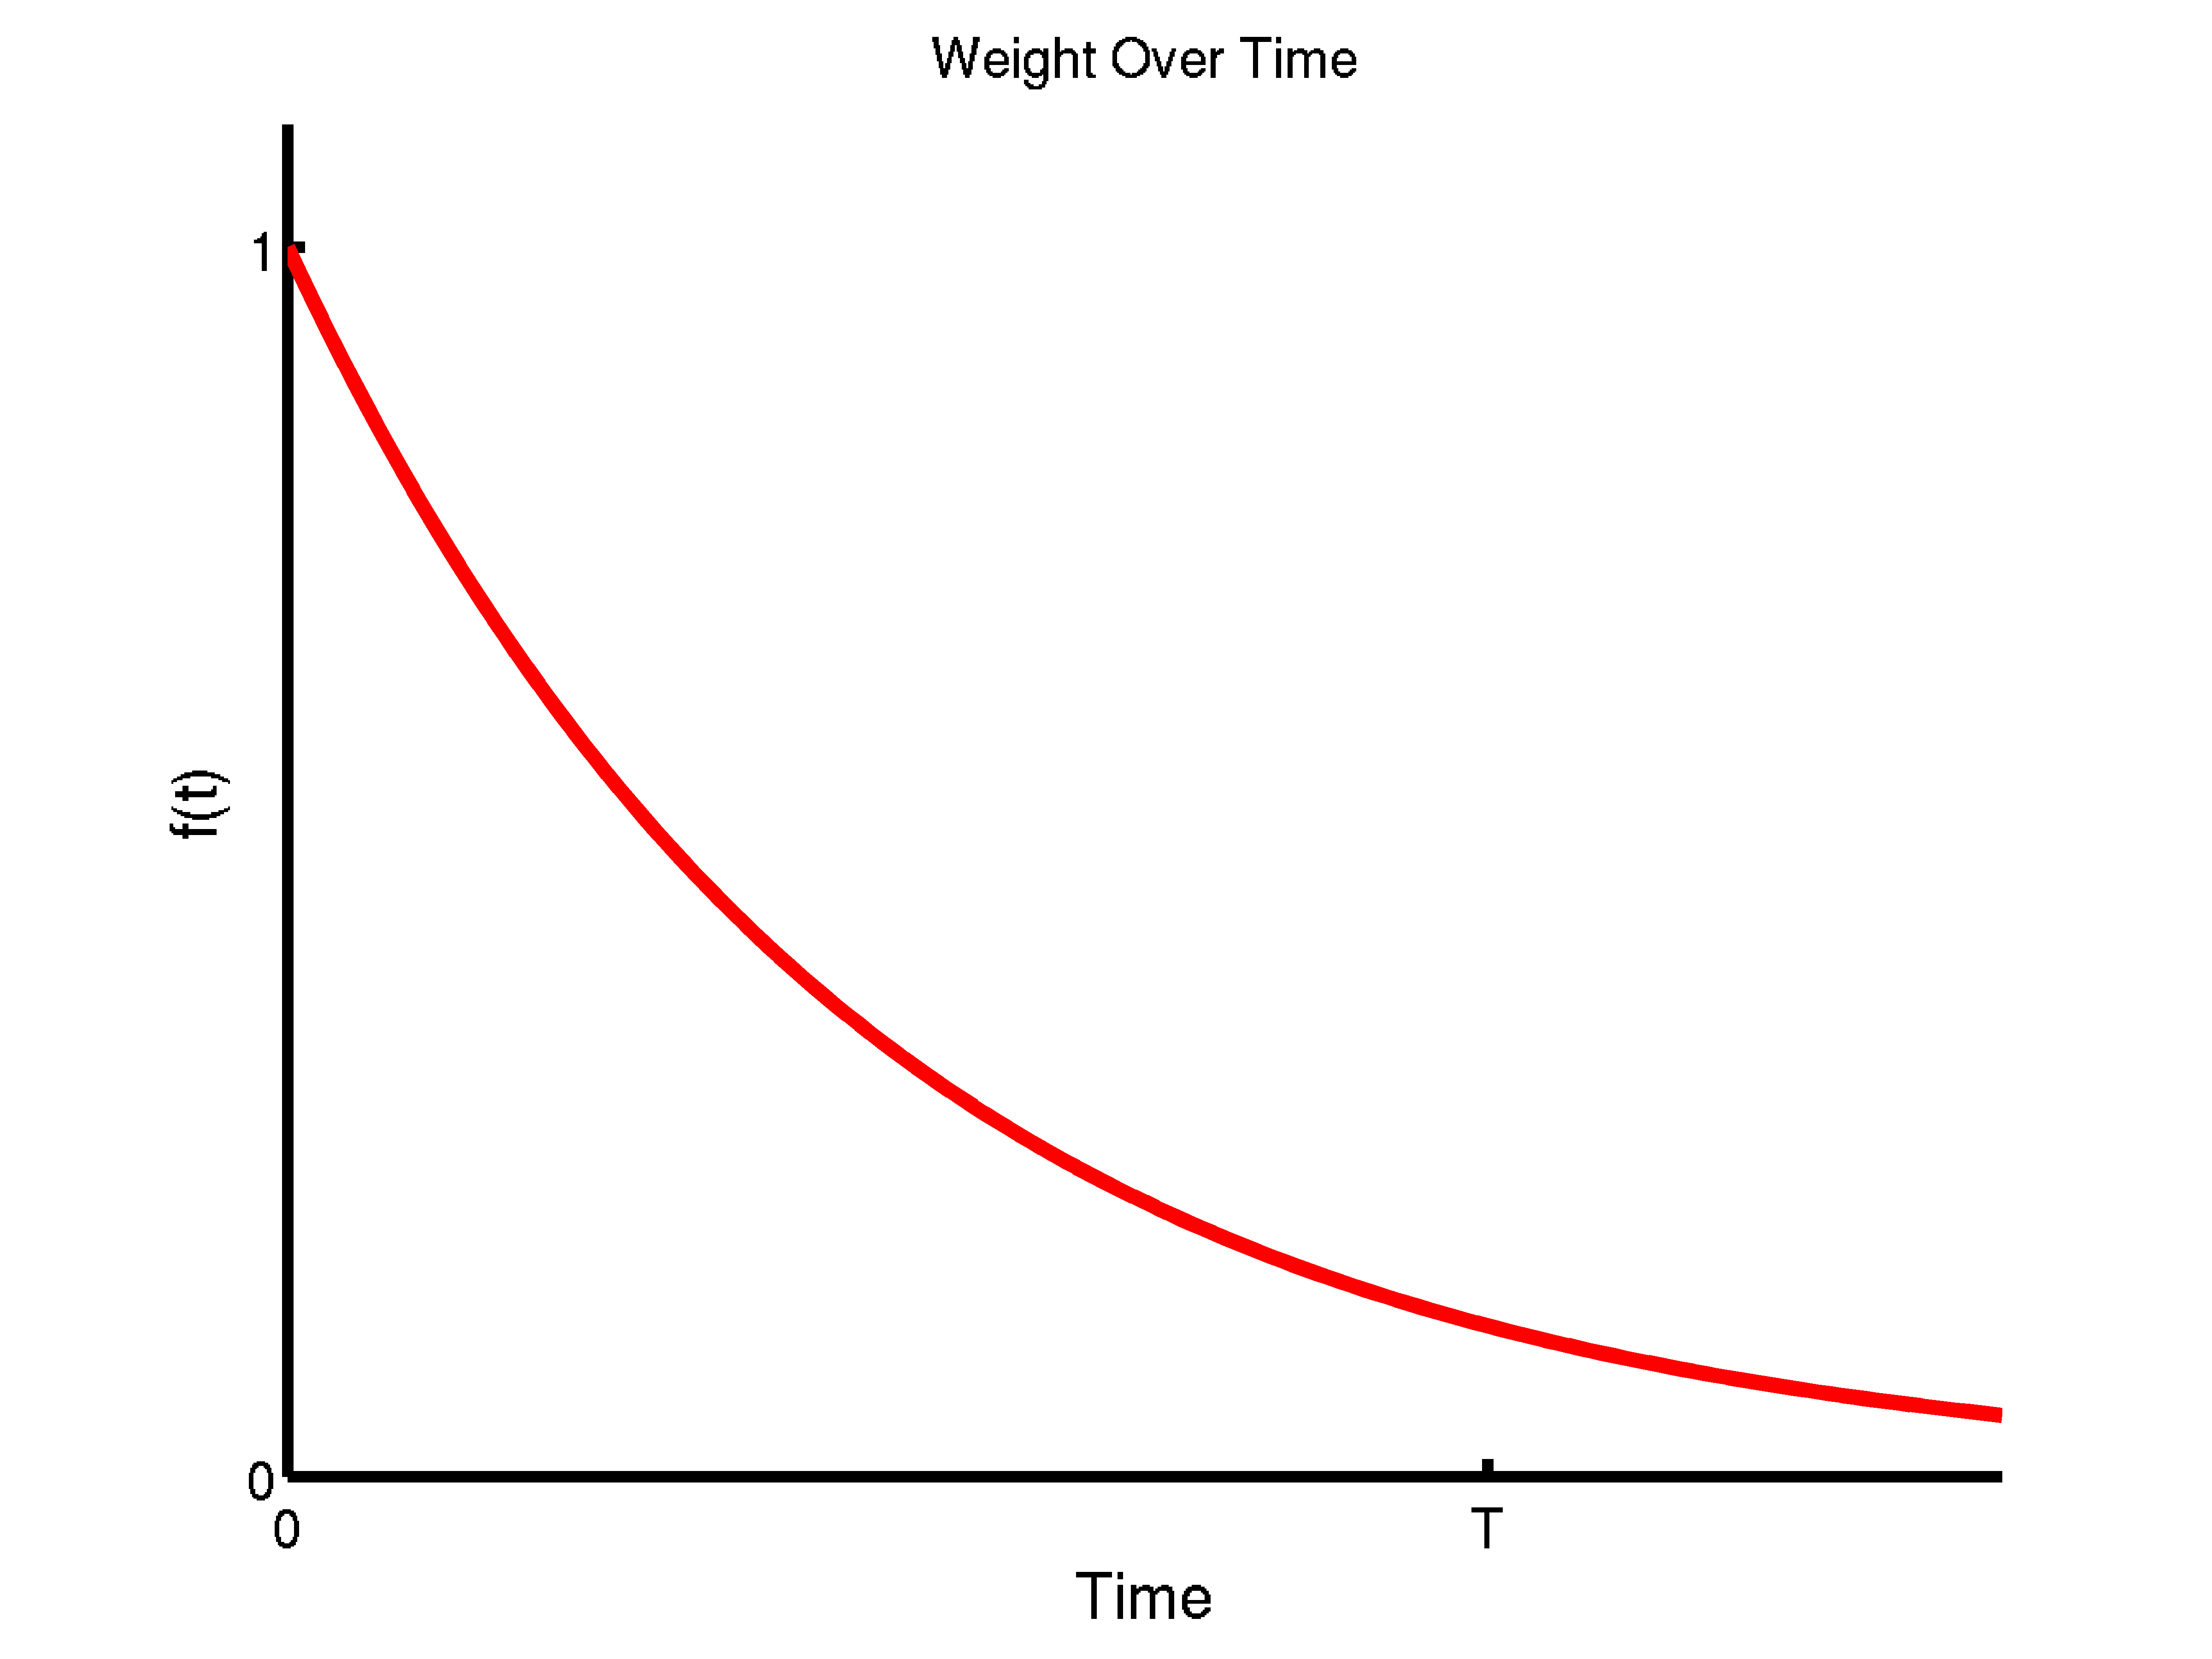
\includegraphics[width=5cm]{img/exponentialDecay}}

    \column{.5\textwidth}
    \vfill

    when you translate it by $f(t-w)$, you shift it and run it
    ``backwards.''
    
    \centerline{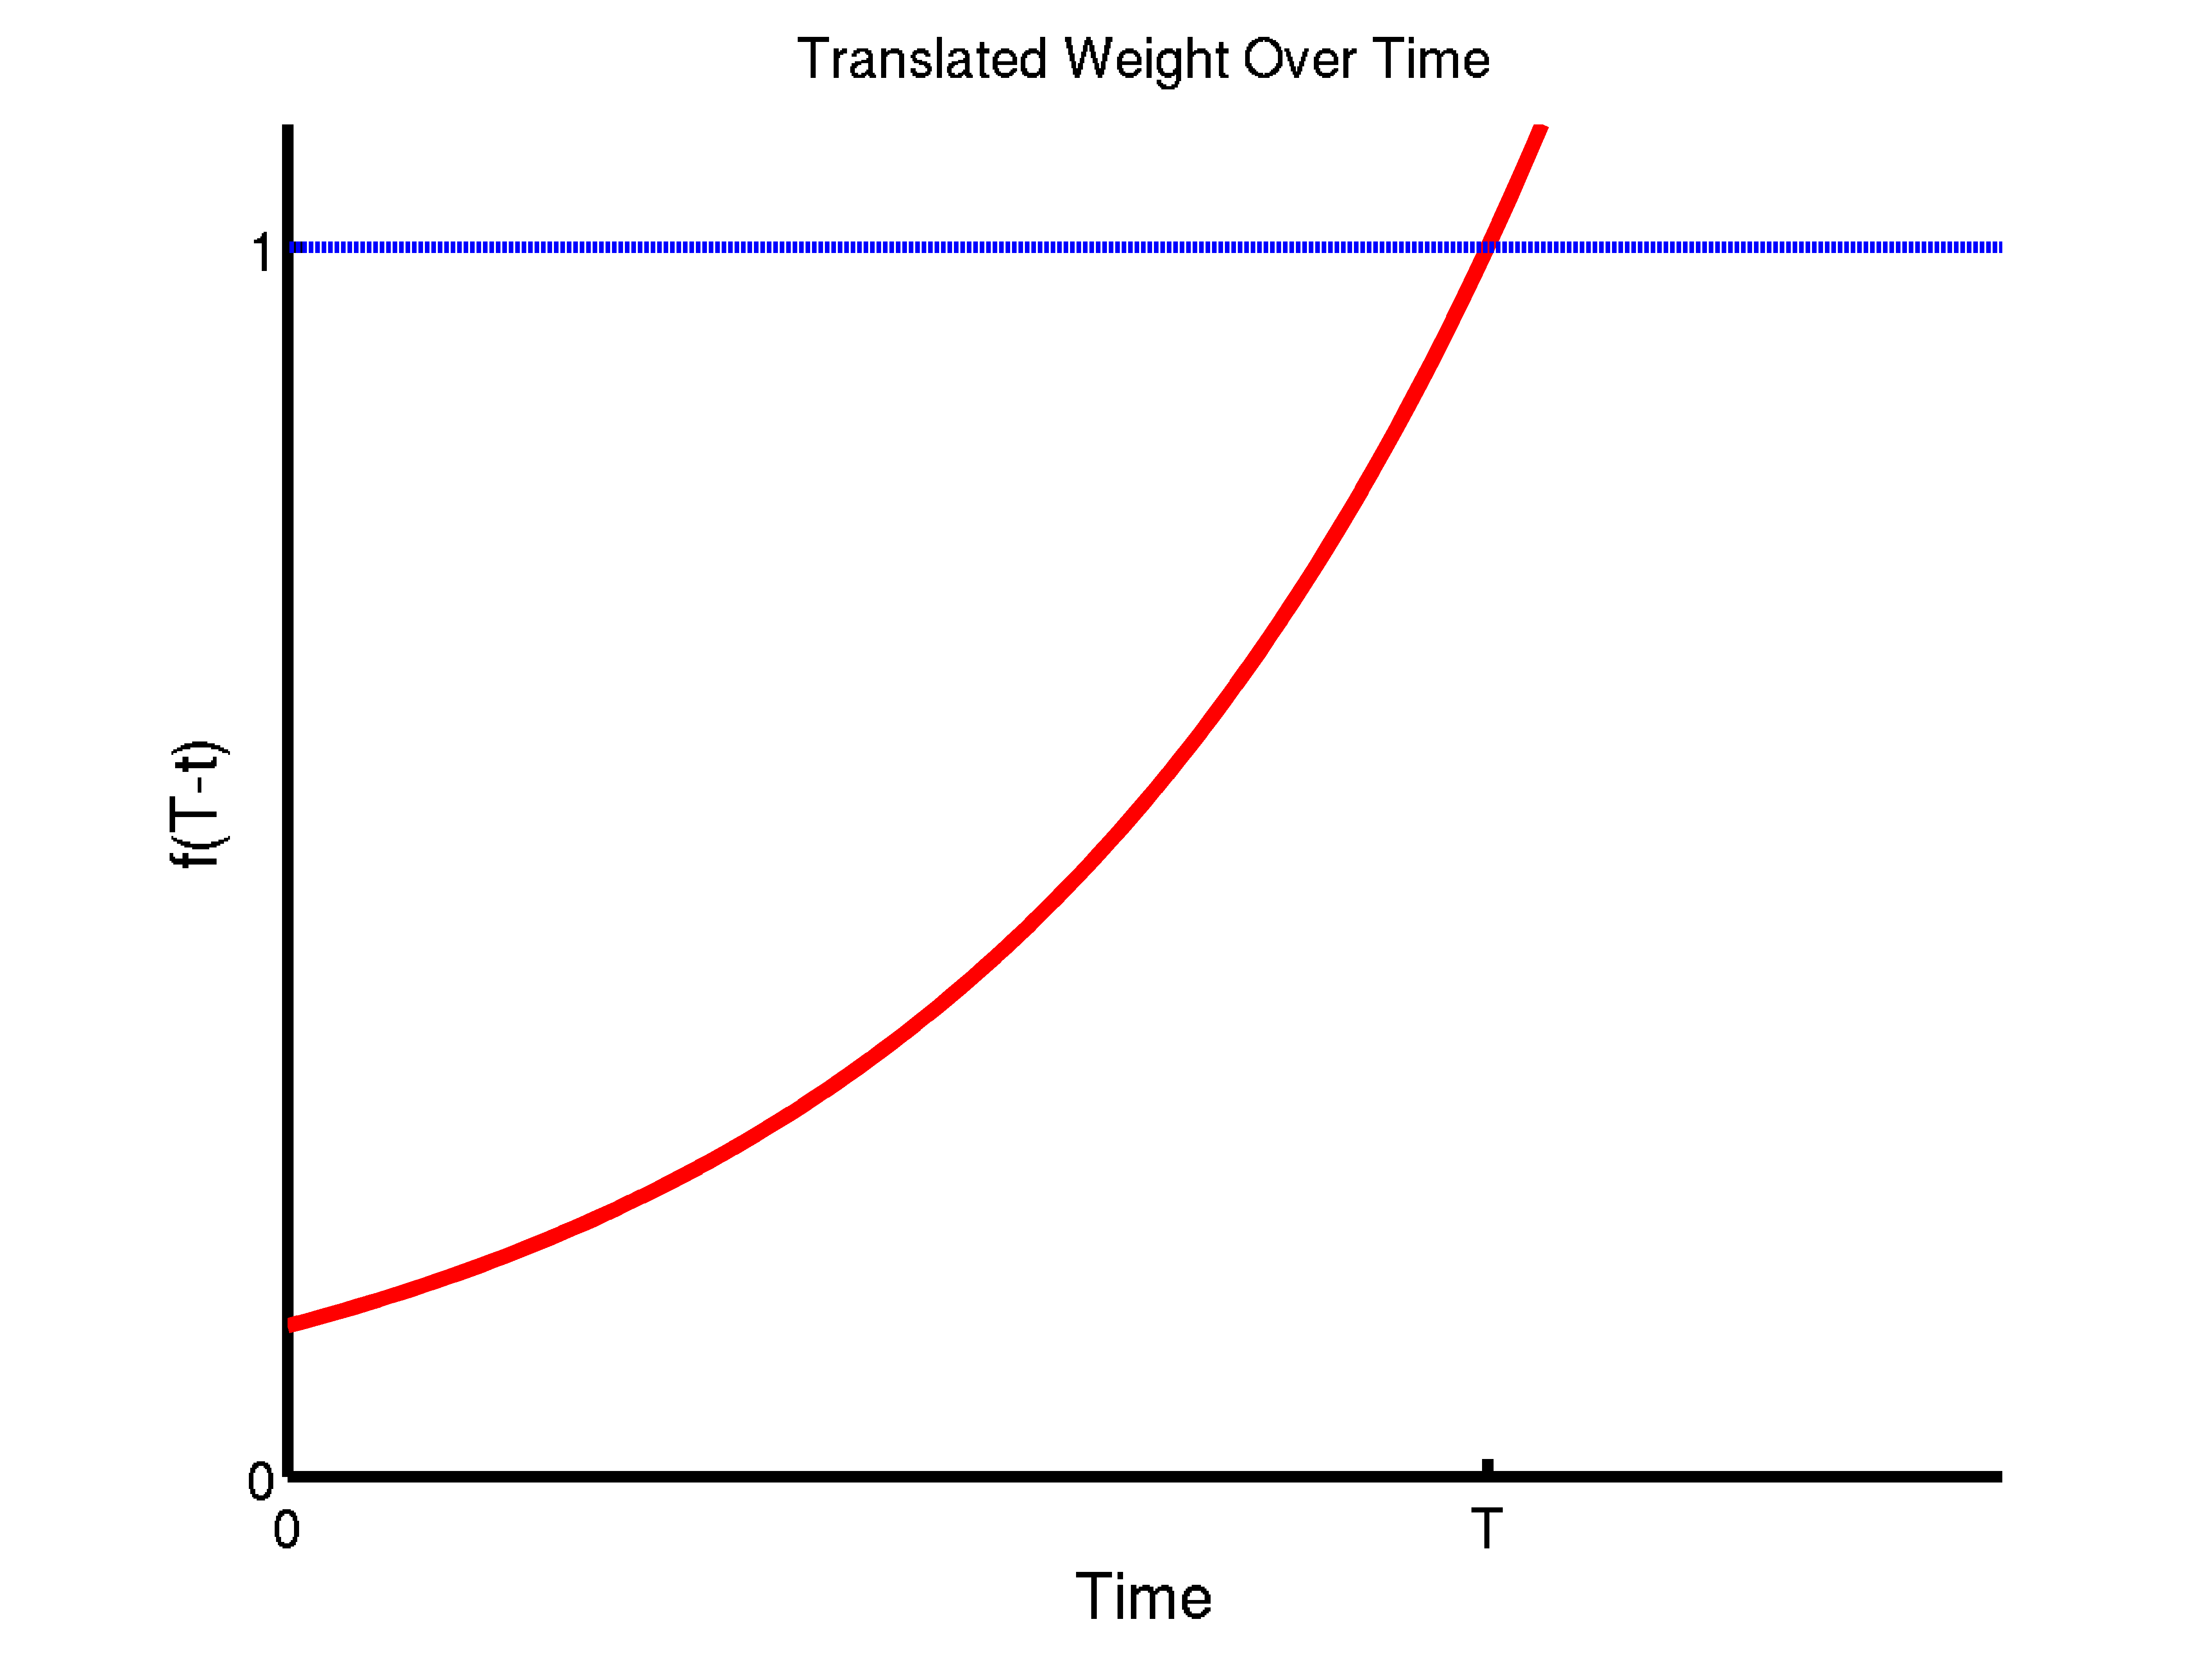
\includegraphics[width=5cm]{img/backwardsExponentialDecay}}

  \end{columns}

\end{frame}

\begin{frame}
  \frametitle{Example}

  Find the convolution $f*g$ for 
  \begin{eqnarray*}
    f(t) & = & e^{-t}, \\
    g(t) & = & t.
  \end{eqnarray*}


  \uncover<2->
  {%

    \begin{columns}
      \column{.3\textwidth}
      \begin{eqnarray*}
        f*g & = & \int^t_0 e^{-(t-w)} w ~ dw, \\
        & = & \int^t_0 e^{-t} e^{w} w ~ dw, \\
        & = & e^{-t} \int^t_0 e^{w} w ~ dw, \\
        & = & e^{-t} \lp t e^t - e^t + 1 \rp, \\
        & = & t - 1 + e^{-t}.
      \end{eqnarray*}

      \column{.7\textwidth}
      \uncover<3->{\centerline{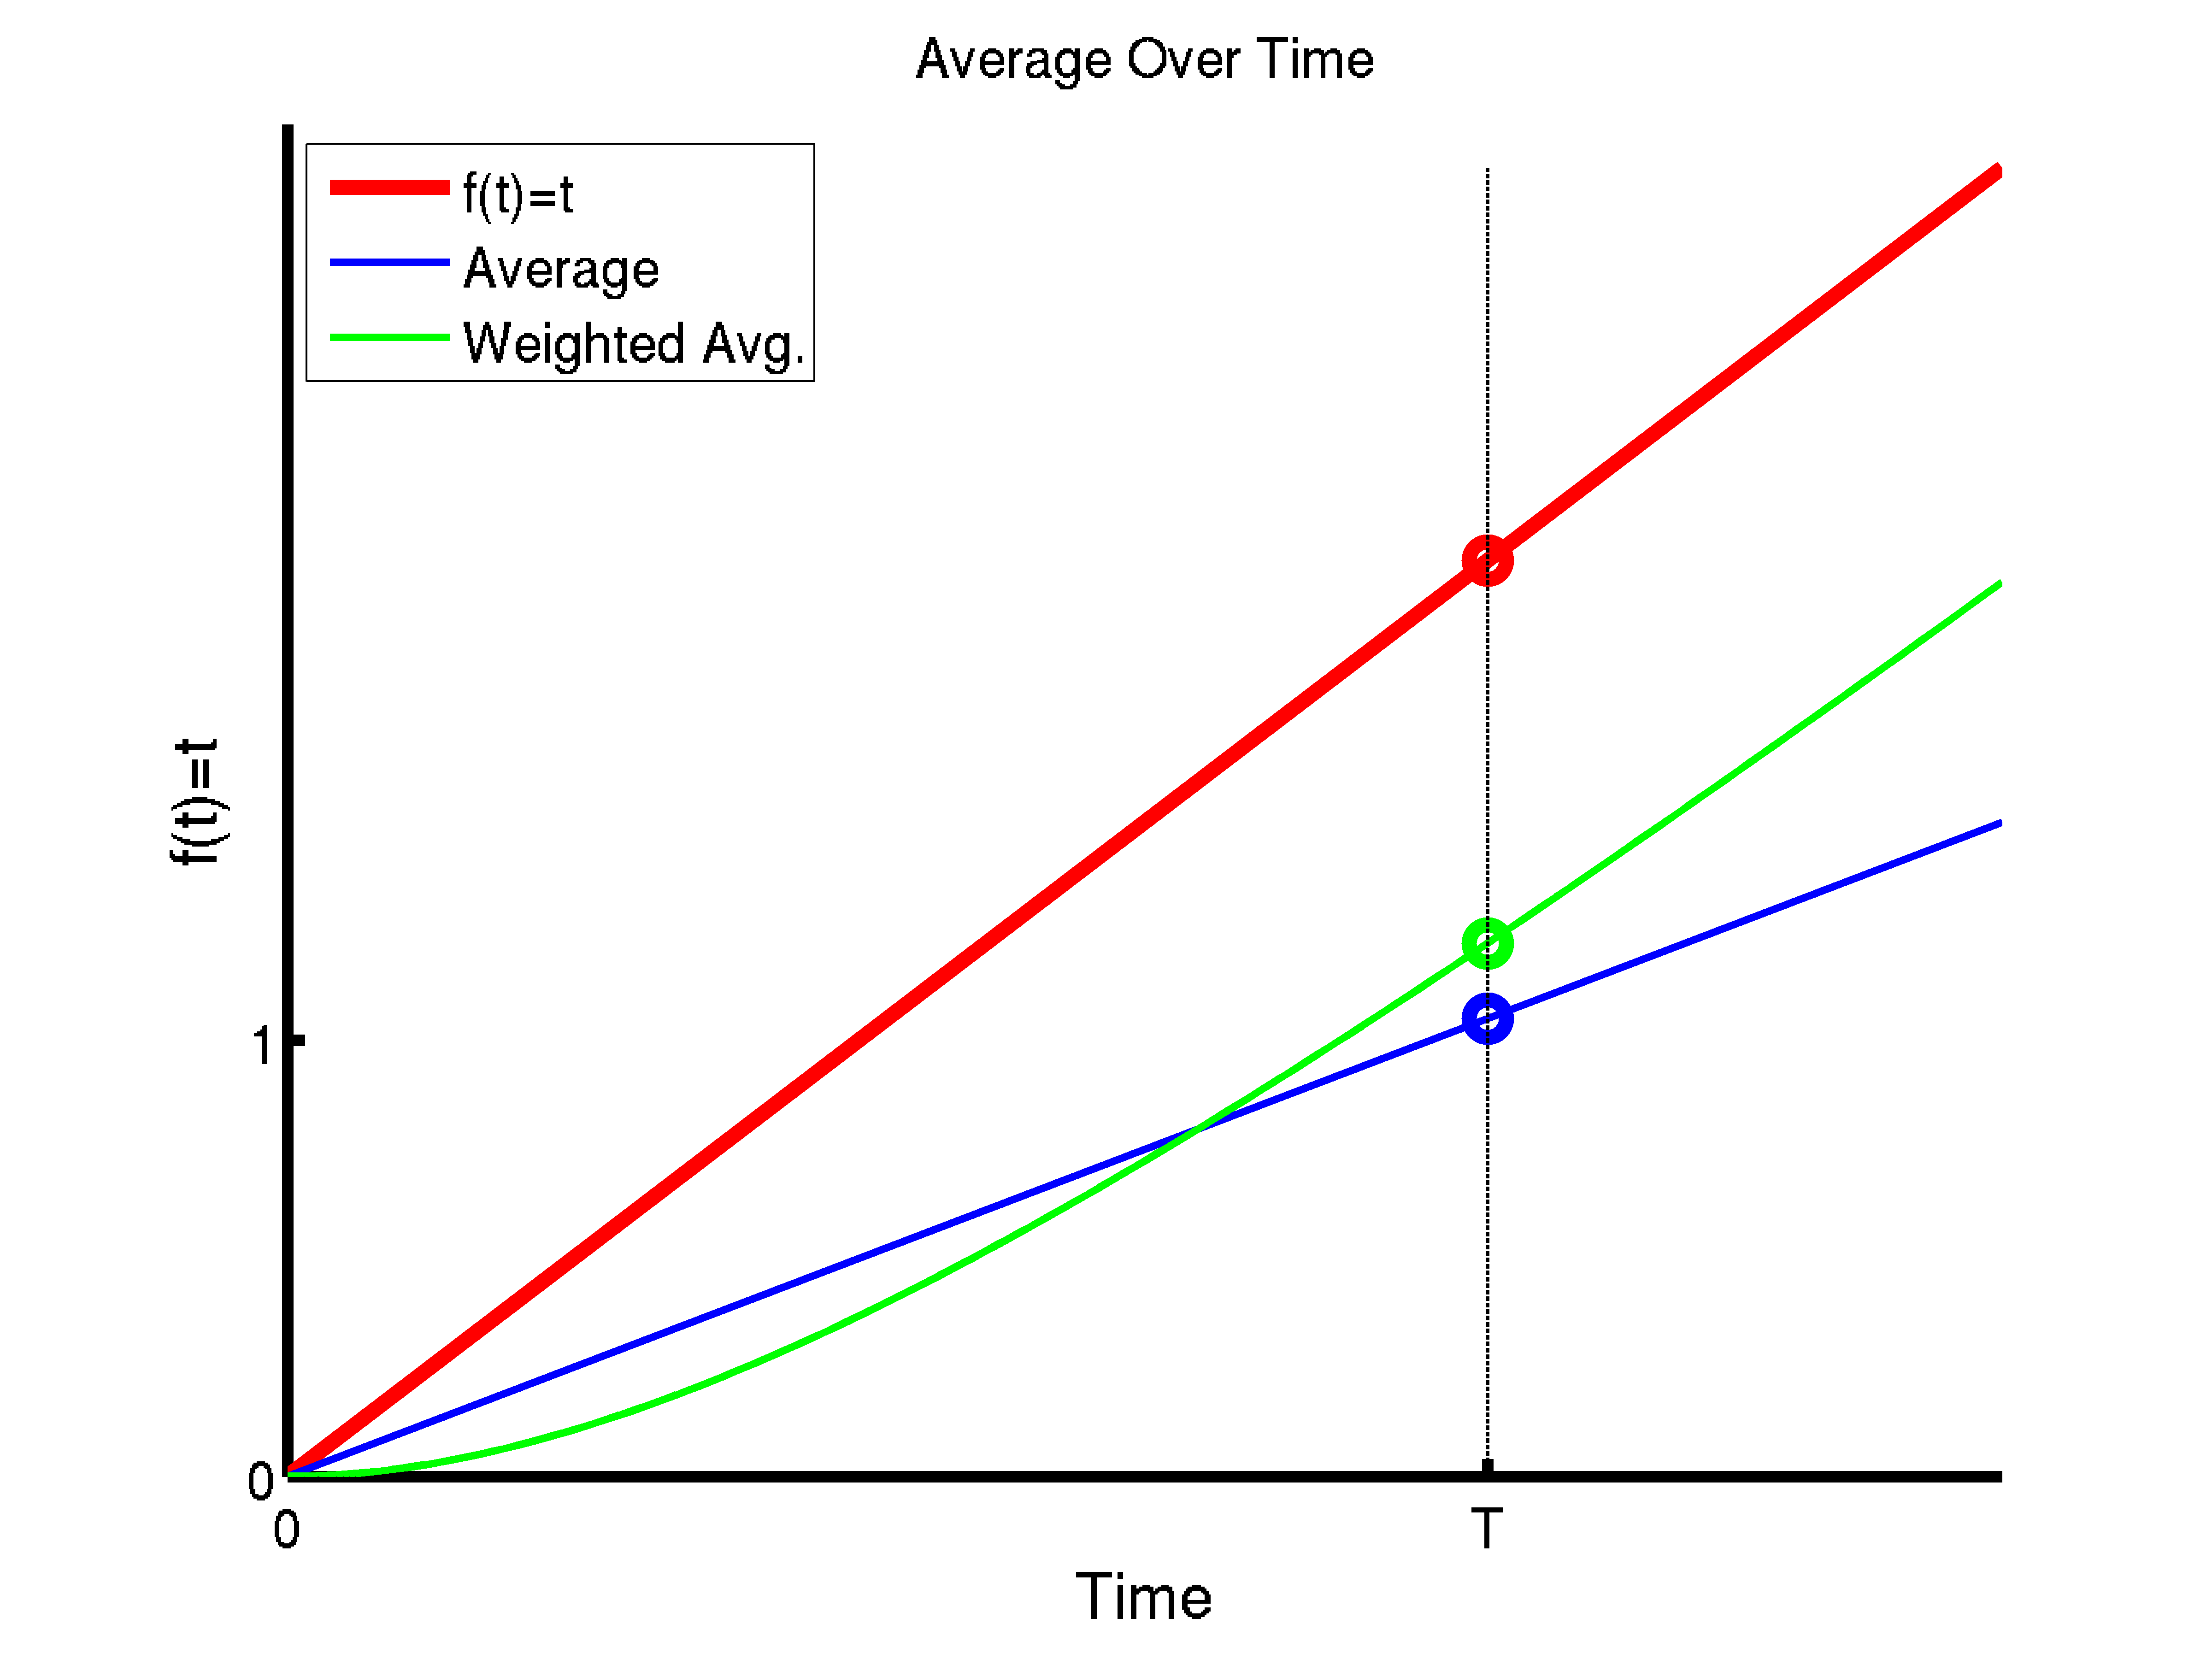
\includegraphics[width=5cm]{img/weightedLinearAverage}}}
    \end{columns}

  }

\end{frame}



\iftoggle{clicker}{%
\begin{frame}
  \frametitle{Clicker Quiz}

   \ifnum\value{clickerQuiz}=1{%
     Determine the Laplace transform of the function $f(t)=te^{4t}$.

     \vspace{2em}
     \begin{tabular}{ll}
       A: & $\frac{1}{(s-4)^2}$ \\ [12pt]
       B: & $\frac{-1}{(s-4)^2}$ \\ [12pt]
       C: & $\frac{1}{(s-4)}$ \\ [12pt]
       D: & $\frac{-1}{(s-4)}$ \\ [12pt]
     \end{tabular}

     \vfill
   }\fi

   \ifnum\value{clickerQuiz}=2{%
     Determine the Laplace transform of the function $f(t)=te^{2t}$.

     \vspace{2em}
     \begin{tabular}{ll}
       A: & $\frac{1}{(s-2)^2}$ \\ [12pt]
       B: & $\frac{-1}{(s-2)^2}$ \\ [12pt]
       C: & $\frac{1}{(s-2)}$ \\ [12pt]
       D: & $\frac{-1}{(s-2)}$ \\ [12pt]
     \end{tabular}

   \vfill
   }\fi

  \ifnum\value{clickerQuiz}=3{%


  \vfill
 }\fi
\end{frame}
}


\subsection{The Laplace Transform of the Convolution}


\begin{frame}
  \frametitle{The Laplace Transform of the Convolution}

  \begin{eqnarray*}
    \laplace{f*g} & = & \int^\infty_0 \int^t_0 f(t-w)g(w) ~ dw ~ dt, \\
    \uncover<2->{& & \mathrm{Calc~III~Magic!}, \\}
    \uncover<3->{& = & \laplace{f}\cdot\laplace{g}.\\}
  \end{eqnarray*}


\end{frame}


\begin{frame}
  \frametitle{Example}

  \vspace*{-3em}
  \begin{eqnarray*}
    f(t) & = & e^{-t}, \\
    g(t) & = & t, \\
    f*g & = & t - 1 + e^{-t}.
  \end{eqnarray*}

  \begin{columns}
  
    \column{.5\textwidth}
    \uncover<2->
    {%

      \begin{eqnarray*}
        \laplace{f*g} & = & \frac{1}{s^2} - \frac{1}{s} + \frac{1}{s+1}.
      \end{eqnarray*}

    }

    \column{.5\textwidth}
    \uncover<3->
    {%

      \begin{eqnarray*}
        \laplace{f} & = & \frac{1}{s+1}, \\
        \laplace{g} & = & \frac{1}{s^2}, \\
        \laplace{f*g} & = & \frac{1}{s^2(s+1)}, \\
        & = & \frac{-1}{s} + \frac{1}{s^2} + \frac{1}{s+1}.
      \end{eqnarray*}

    }

  \end{columns}

  \vfill
  
\end{frame}


\begin{frame}
  \frametitle{Solving Differential Equations}

  \begin{eqnarray*}
    y'-y & = & e^{-t}, \\
    y(0) & = & 0.
  \end{eqnarray*}

  \uncover<2>
  {
    \begin{eqnarray*}
      -y(0) + s \laplace{y} - \laplace{y} & = & \frac{1}{s+1}, \\
      (s-1) \laplace{y} & = & \frac{1}{s+1}, \\
      \laplace{y} & = & \frac{1}{s-1}\cdot\frac{1}{s+1}.
    \end{eqnarray*}
  }


\end{frame}


\begin{frame}
  \frametitle{Solving Differential Equations}

  \begin{columns}
    \column{.5\textwidth}
    \begin{eqnarray*}
      \laplace{y} & = & \frac{1}{s-1}\cdot\frac{1}{s+1}.
    \end{eqnarray*}

    \column{.5\textwidth}
    \only<2->
    {
      \begin{eqnarray*}
        \begin{array}{rclcl}
          \laplace{e^t}   & = & \frac{1}{s-1} & = & f  \\
          \laplace{e^{-t}} & = & \frac{1}{s+1} & = & g,
        \end{array}
      \end{eqnarray*}
    }
    \only<3->
    {
      \begin{eqnarray*}
        \Rightarrow y & = & f*g, \\
        & = & \int^t_0 e^{t-w} e^{-w} ~ dw, \\
        & = & e^{t} \int^t_0 e^{-w} e^{-w} ~ dw, \\
        & = & e^t \lp -\half e^{-2w} \bigg|^t_0 \rp, \\
        & = & e^t \lp -\half e^{2t} + \half \rp, \\
        & = & -\half e^{-t} + \half e^{t}.
      \end{eqnarray*}
    }

    
  \end{columns}


\end{frame}


\begin{frame}
  \frametitle{Example}

  \begin{eqnarray*}
    y''+4y & = & \cos(2t), \\
    y(0) & = & 0, \\
    y'(0) & = & 0.
  \end{eqnarray*}

  \uncover<2->
  {
    \begin{eqnarray*}
      -y'(0) - sy(0) + s^2 \laplace{y} + 4 \laplace{y} & = & \frac{s}{s^2+4}, \\
      \laplace{y} & = & \frac{1}{s^2+4} \cdot \frac{s}{s^2+4}.
    \end{eqnarray*}
  }

  \uncover<3->
  {
    \begin{itemize}
    \item $\laplace{y} =  -\half \deriv{~}{s} \lp s^2+4 \rp^{-1}$ ~
      $\Rightarrow~y=\half t \sin(2t)$
    \item $y=\half\int^t_0 \sin(2(t-w))\cos(w)~dw.$
    \end{itemize}
  }

\end{frame}


\begin{frame}
  \frametitle{Example}

  % image of a circuit

  \uncover<2->
  {
    \begin{eqnarray*}
      R q' + \frac{q}{C} & = & v(t), \\
      q(0) & = & 0.
    \end{eqnarray*}
  }

\end{frame}

\begin{frame}
  \frametitle{Example}

    \begin{eqnarray*}
      R q' + \frac{q}{C} & = & v(t), \\
      q(0) & = & 0.
    \end{eqnarray*}

  \uncover<2->
  {
    Take the Laplace transform:
    \begin{eqnarray*}
      -R q(0) + Rs\laplace{q} + \frac{1}{C} \laplace{q} & = & \laplace{v}, \\
      \lp Rs+\frac{1}{C} \rp \laplace{q}  & = & \laplace{v}, \\
      \laplace{q}  & = & \frac{1}{Rs+\frac{1}{C}} \laplace{v}, \\
      & = & \frac{1}{R} \frac{1}{s + \frac{1}{RC}} \laplace{v}.
    \end{eqnarray*}
  }


\end{frame}


\begin{frame}
  \frametitle{Example}

  % image of a circuit

    Take the Laplace transform:
    \begin{eqnarray*}
      \laplace{q}  & = & \frac{1}{R} \frac{1}{s + \frac{1}{RC}} \laplace{v}.
    \end{eqnarray*}

  \uncover<2->
  {

    \begin{eqnarray*}
      y & = & \frac{1}{R} \int^t_0 e^{-(t-w)/(RC)} v(w) ~ dw, \\
      & = & \frac{1}{R} e^{-t/(RC)} \int^t_0 e^{w/(RC)} v(w) ~ dw.
    \end{eqnarray*}

  }


\end{frame}




% LocalWords:  Clarkson pausesection hideothersubsections
